\section{Ekonomická optimalizácia}
V tejto časti zhrnieme hlavný cieľ tejto práce a to optimalizáciu prietokového biochemického reaktora pomocou hybridného modelovania s využitím metódy garantovaného odhadu parametrov. Ukážeme, na akom princípe bude takýto hybridný model fungovať a porovnáme ho s inými metódami, ktoré sa tak isto vedia vysporiadať s úlohou optimalizácie zariadenia. Najskôr, však potrebujeme zadefinovať problematiku.

Majme fiktívne zariadenie prietokového biochemického reaktora, ktoré vieme simulovať Monod modelom. Parametre tohto modelu, ako aj ich veľkosť, sú uvedené v Tabuľke \ref{tab:case_study_monod_params}. Našim cenným produktom bude samotná biomasa (napr. pekárenské droždie), takže sa budeme snažiť maximalizovať produkciu biomasy, ale na druhej strane budeme požadovať, aby sme pri tom minuli čo najmenej substrátu. Ak túto vetu transformujeme na matematický opis, mohli by sme získať takúto optimalizačnú úlohu
\begin{equation}
	\label{eq:chemostat_opt_general}
	\begin{split}
		\min_{D} &\quad D\left(1-\bar{x}\right), \\
		\text{s.t.} &\quad \bar{x} = f(D,\bar{s})
	\end{split}
\end{equation}
kde $ \bar{x} $ je ustálený stav koncentrácie biomasy a $ \bar{s} $ je ustálený stav koncentrácie substrátu. Funkcia $ f(D,\bar{s}) $ vyjadruje vzťah medzi hodnotou ustáleného stavu koncentrácie biomasy, substrátu a rýchlosti riedenia. Funkciu $ f(D,\bar{s}) $ získame z mechanického modelu, ktorým sme opísali správanie nášho zariadenia. Tento model predstavuje Haldane model resp. model s inhibíciou, ktorého parametre sú tak isto uvedené v Tabuľke \ref{tab:case_study_monod_params}. 

\begin{table}
	\centering
	\caption{Nastavenie parametrov Monod a Haldane modelu.}
	\label{tab:case_study_monod_params}
	\begin{tabular}{lll}
		\hline
		\textbf{Parameter} & \textbf{Symbol} & \textbf{Veľkosť} \\
		\hline
		Maximálna špecifická rýchlosť rastu & $\mu_{m}$ & 0.53\si{\per\hour} \\
		Michaelisova konštanta & $K_{M}$ & 1.20\si{\gram\per\liter} \\
		Rýchlosť tvorby produktu & $ \nu $ & 0.50\si{\per\hour} \\
		Výťažok (biomasa) & $Y_{x}$ & 0.40\\
		Výťažok (produkt) & $Y_{p}$ & 1.00\\
		Objem reaktora & $V$ & 3.33\si{\liter} \\
		Prietok substrátu/suspenzie & $F$ & 1.00\si{\liter\per\hour} \\
		Koncentrácia substrátu na vstupe & $s_{in}$ & 20.00\si{\gram\per\liter} \\
		Koeficient inhibície & $ K_{I} $ & 70.00\si{\gram\per\liter}\\
		\hline
	\end{tabular}
\end{table}

Ustálený stav Haldane modelu môžeme napísať v tvare
\begin{align}
	&0 = \left(\mu(\bar{s}) - D\right)\bar{x}, \label{eq:tmp_haldane_x_ss}\\
	&0 = D\left(s_{in} - \bar{s}\right) - \frac{1}{Y_{x}}\mu(\bar{s})\bar{x} - \frac{1}{Y_{p}}\nu \bar{x}, \label{eq:tmp_haldane_s_ss}\\
	&0 = \nu \bar{x} - D\bar{p} \label{eq:tmp_haldane_p_ss}.
\end{align}
Z rovnice \eqref{eq:tmp_haldane_x_ss} sme získali dve riešenia -- triviálne, ak koncentrácia biomasy bude v každom čase nulová; netriviálne, ak špecifická rýchlosť rastu bude rovná rýchlosti riedenia. Potom pre špecifickú rýchlosť rastu môžeme písať 
\begin{equation}
	\mu(\bar{s}) = D = \mu_{m}\frac{\bar{s}}{K_{M} + \bar{s} + \frac{\bar{s}^2}{K_{I}}} \quad \Longrightarrow \quad
	\frac{D}{K_{I}}\bar{s}^2 + (D-\mu_{m})\bar{s} + DK_{M} = 0.
\end{equation}
Riešením tejto kvadratickej rovnice dostaneme dve riešenia, pričom fyzikálny zmysel má iba jedno
\begin{equation}
	\label{eq:haldane_subs_ss}
	\bar{s} = -K_{I}\frac{\left(D-\mu_{m}\right) + \sqrt{\left(D-\mu_{m}\right)^2 - 4\frac{D^2}{K_{I}}K_{M}}}{2D}. 
\end{equation}
Takto sme získali rovnicu ustáleného stavu koncentrácie substrátu. Ustálený stav koncentrácie biomasy vieme odvodiť z rovnice \eqref{eq:tmp_haldane_s_ss}
\begin{equation}
\label{eq:haldane_biomass_ss}
	0 = D\left(s_{in}-\bar{s}\right) - \left(\frac{1}{Y_{x}}D + \frac{1}{Y_{p}}\nu\right)\bar{x} \quad \Longrightarrow \quad
	\bar{x} = \frac{D\left(s_{in}-\bar{s}\right)}{\frac{1}{Y_{x}}D + \frac{1}{Y_{x}}\nu}. 
\end{equation}
A nakoniec posledná rovnica \eqref{eq:tmp_haldane_p_ss} definuje hodnotu ustáleného stavu produktu
\begin{equation}
\label{eq:haldane_product_ss}
	0 = \nu \bar{x} - D\bar{p} \quad \Longrightarrow \quad \bar{p} = \frac{\nu}{D}\bar{x}.
\end{equation}
Keďže už vieme aký predpis má funkcia $ f(D,\bar{s}) $, môžeme optimalizačnú úlohu \eqref{eq:chemostat_opt_general} upraviť do nasledujúceho tvaru 
\begin{equation}
\label{eq:chemostat_opt_w_ss}
	 \begin{split}
		 \min_{D} &\quad D\left(1-\alpha\bar{x}\right), \\
		 \text{s.t.} &\quad \bar{x} = \frac{D\left(s_{in}-\bar{s}\right)}{\frac{1}{Y_{x}}D + \frac{1}{Y_{x}}\nu} \\
		 &\quad \bar{s} = -K_{I}\frac{\left(D-\mu_{m}\right) + \sqrt{\left(D-\mu_{m}\right)^2 - 4\frac{D^2}{K_{I}}K_{M}}}{2D}
	 \end{split}
\end{equation}
Kvôli problémom s definičným oborom účelovej funkcie Haldane modelu (viď rovnicu \eqref{eq:haldane_subs_ss}), sme museli pridať do účelovej funkcie koeficient $ \alpha $, ktorého veľkosť sme empiricky zvolili rovný $ \alpha = 0.5 $. Toto nám umožnilo rozšíriť definičný obor aspoň po oblasť optimálnej hodnoty Monod modelu.

Treba zdôrazniť, že správanie takto nastaveného Haldane modelu je naprosto odlišné od nášho zariadenia, pretože za určitých podmienok sa prejavuje inhibícia v dôsledku vysokej koncentrácie substrátu, a preto bude mať optimum účelovej funkcie niekde inde ako naše zariadenie simulované Monod modelom, ako to vidno na Obr. \ref{fig:cost_fun_comparison}. To znamená, že ak by sme sa riadili iba týmto nepresným mechanickým modelom, naše zariadenie by vôbec nepracovalo najefektívnejšie ako to je len možné. Z tohto dôvodu sa budeme snažiť navrhnúť hybridný model tak, aby dokázal vyrovnať rozdiel medzi nominálnym modelom a zariadením. Vhodnou štruktúrou hybridného modelu na riešenie tejto problematiky je paralelné zapojenie.

\begin{figure}
	\centering
	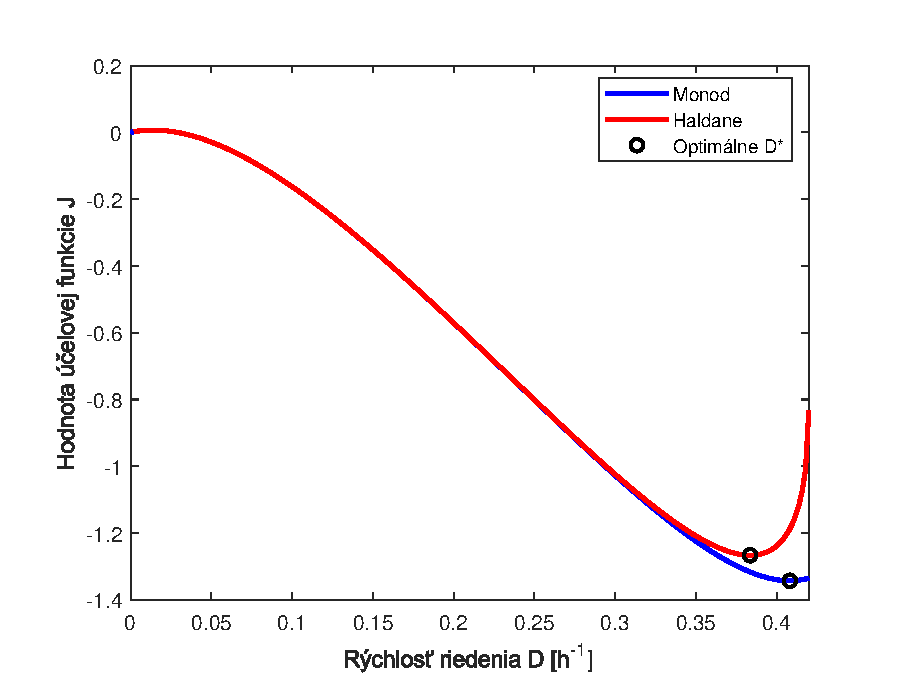
\includegraphics[width=0.7\linewidth]{images/cost_fun_comparison}
	\caption{Porovnanie účelovej funkcie Monod a Haldane modelu. Zariadenie je simulované Monod modelom a Haldane model predstavuje náš nepresný mechanický model.}
	\label{fig:cost_fun_comparison}
\end{figure}

\textbf{Použitie hybridných modelov.} Na začiatku treba spomenúť, že ide o iteračnú metódu, i keď hybridné modely majú tú výhodu, že dátovú časť by sme vedeli natrénovať na údajoch zo zariadenia aj bez iteračného prístupu, ale nemali by sme zaručenú úspešnosť výsledku. 

Princíp optimalizácie demonštrujeme na situácii, keď dokážeme merať iba koncentráciu substrátu. Z ustáleného stavu, spravíme skokovú zmenu v rýchlosti zrieďovania $ D $, v prípade zariadenia aj modelu. Na základe rozdielu $ \Delta_{s} $ týchto dát
\begin{equation}
	\Delta_{s} = \tilde{s} - s,
\end{equation}
kde $ \tilde{s} $ sú údaje získané zo zariadenia a $ s $ predstavuje údaje z nominálneho modelu, identifikujeme dátový model pomocou metódy GOP. V prípade, že by našim dátovým modelom bol FIR, môžeme využiť rovnice \eqref{eq:gpe_fir_min_rad} a \eqref{eq:gpe_fir_param_est}. ARX model by sme mohli identifikovať pomocou \eqref{eq:gpe_arx_min_rad} a \eqref{eq:gpe_arx_param_est}. Takto natrénovaný dátový model využijeme na korekciu ustáleného stavu substrátu nominálneho modelu v optimalizačnej úlohe \eqref{eq:chemostat_opt_w_ss}. Po úprave by sme ju mohli formulovať nasledovne
\begin{equation}
\label{eq:hybrid_opt_subs}
	\begin{split}
		\min_{D} &\quad D\left(1-\alpha\bar{x}\right), \\
		\text{s.t.} &\quad \bar{x} = \frac{D\left(s_{in}-s_{corr}\right)}{\frac{1}{Y_{x}}D + \frac{1}{Y_{x}}\nu} \\
		&\quad s_{corr} = \bar{\Delta}_{s}(D) + \bar{s}\\
		&\quad \bar{s} = -K_{I}\frac{\left(D-\mu_{m}\right) + \sqrt{\left(D-\mu_{m}\right)^2 - 4\frac{D^2}{K_{I}}K_{M}}}{2D}
	\end{split}
\end{equation}
kde $ \bar{\Delta}_{s}(D) $ je ustálený stav dátového modelu. Riešenie tejto upravenej optimalizačnej úlohy nám vráti novú hodnotu optimálneho $ D $, odlišnú od predchádzajúcej a túto využijeme na generovanie novej skokovej zmeny, nových dát. 

Takto postupujeme, až dokým neskonvergujeme k optimálnej hodnote rýchlosti riedenia $ D^{\star} $ zariadenia. V tomto bode by ustálený stav dátového modelu $ \bar{\Delta}_s $ mal nadobudnúť hodnotu
\begin{equation}
	\bar{\Delta}_s = \hat{s}\left(D^{\star}\right) - \bar{s}\left(D^{\star}\right),
\end{equation} 
kde $ \hat{s}\left(D^{\star}\right) $ je hodnota ustáleného stavu koncentrácie substrátu zariadenia a $ \bar{s}\left(D^{\star}\right) $ nominálneho modelu pri rýchlosti riedenia $ D^{\star} $.

Ak by nastala situácia, že zo zariadenia vieme získať iba údaje o koncentrácii biomasy, princíp fungovania hybridného modelu by sa nezmenil. Zmenili by sa iba dáta resp. dátové modely. Zaznamenali by sme rozdiel v koncentrácii biomasy $ \Delta_{x} $ a pripravili trénovacie dáta ako
\begin{equation}
	\Delta_{x} = \tilde{x} - x,
\end{equation} 
kde $ \tilde{x} $ sú namerané údaje zo zariadenia a $ x $ sú dáta z nominálneho modelu. Na základe týchto údajov by sme identifikovali dátový model, ktorý by sme použili na úpravu ustáleného stavu biomasy $ \bar{x} $ nominálneho modelu v optimalizačnej úlohe nasledovným spôsobom
\begin{equation}
\label{eq:hybrid_opt_bio}
	\begin{split}
		\min_{D} &\quad D\left(1-\alpha\left(\bar{x}+\bar{\Delta}_{x}(D)\right)\right), \\
		\text{s.t.} &\quad \bar{x} = \frac{D\left(s_{in}-\bar{s}\right)}{\frac{1}{Y_{x}}D + \frac{1}{Y_{x}}\nu} \\
		&\quad \bar{s} = -K_{I}\frac{\left(D-\mu_{m}\right) + \sqrt{\left(D-\mu_{m}\right)^2 - 4\frac{D^2}{K_{I}}K_{M}}}{2D}
	\end{split}
\end{equation}
kde $ \bar{\Delta}_{x}(D) $ predstavuje ustálený stav dátového modelu.

Avšak, medzi dátami o koncentrácii substrátu a biomasy je kvalitatívny rozdiel, a tým je vplyv šumu merania. Zatiaľ čo, meranie koncentrácie substrátu nebýva zaťažené veľkou chybou merania, koncentrácia biomasy má výrazne vyššiu fluktuáciu. Preto sa najčastejšie z výstupných prúdov meria koncentrácia substrátu. 

Aby sme vedeli zhodnotiť kvalitu prístupu k optimalizácii nášho zariadenia použitím hybridných modelov, porovnáme tento prístup s ďalšími dvoma metódami. Sú nimi dvojkroková optimalizácia a schéma úpravy modifikátora. Oba tieto prístupy patria k iteračným metódam.

\textbf{Dvojkroková optimalizácia.}
V prvej fáze sa zameriame na odhad parametrov nominálneho modelu. Treba si uvedomiť, že nepotrebujeme odhadovať všetky parametre modelu, pretože niektoré z nich vieme získať meraním ako jednotlivé výťažky $ Y_{x}, Y_{p} $, rýchlosť tvorby produktu $ \nu $, koncentráciu substrátu na vstupe $ s_{in} $. Tieto parametre si vopred zadefinujeme a budú mať takú veľkosť, ako udáva Tabuľka \ref{tab:case_study_monod_params}. Zvyšné parametre modelu, maximálnu špecifickú rýchlosť rastu $ \mu_{m} $, Michaelisovu konštantu $ K_{M} $ a koeficient inhibície $ K_{I} $, tzv. kinetické členy, budeme odhadovať. Na základe nameraných údajov zo skokovej zmeny môžeme zvoliť dve cesty.

V prípade, že disponujeme dátami koncentrácie biomasy aj substrátu, môžeme optimalizačný problém odhadu parametrov sformulovať nasledovne
\begin{equation}
\label{eq:twostep_der_app}
	\begin{split}
		\min_{\mu_{m},K_{M}} \quad &\sum_{i=1}^{N} \left(\Delta_{i} - \left(\mu(\tilde{s}_{i}) - D\right)\tilde{x}_{i}\right)^2, \\
		\text{s.t.} \quad &\Delta_{i} = \frac{\tilde{x}_{i} - \tilde{x}_{i-1}}{t_{i} - t_{i-1}} \\
		\quad &\mu(\tilde{s}_{i})=\mu_{m}\frac{\tilde{s}_{i}}{K_{M} + \tilde{s}_{i} + \frac{\tilde{s}_{i}^2}{K_{I}}}
	\end{split}
\end{equation} 
pre všetky $ i \in \lbrace 1,2,3,\dots,N \rbrace $, kde $ \tilde{x}_{i} $ predstavuje nameranú hodnotu koncentrácie biomasy v $ i $--tom kroku v čase $ t_i $, $ \tilde{s}_{i} $ substrátu a $ \Delta_{i} $ predstavuje spätnú diferenciu v $ i $--tom kroku. Táto metóda aproximuje údaje o derivácii časového priebehu koncentrácie biomasy. Najväčšou prekážkou pre takýto prístup je samotný šum merania a čím väčší bude jeho rozptyl, tým ďalej budeme od skutočnej derivácie.

Druhý prístup odhaduje parametre samotných diferenciálnych rovníc nominálneho modelu na základe nameraných údajov koncentrácie substrátu $ \tilde{s} $. Zatiaľ čo formulácia optimalizačného problému sa príliš nezmení, zložitosť výpočtu sa výrazne zvýši. V tomto prípade je nutné, v každom nameranom bode, niekoľkokrát numericky vyhodnotiť priebehy koncentrácie biomasy aj substrátu a porovnať ich s nameraným signálom  tak, aby sme získali optimálne riešenie. Túto problematiku by sme mohli sformulovať následovne
\begin{equation}
\label{eq:twostep_diff_pe}
	\begin{split}
		\min_{\mu_{m},K_{M}} \quad & \sum_{i=1}^{N} \left(\tilde{s}_{i}-s_{i}\right)^2, \\
		\textrm{s.t.} \quad & \dot{s} = D(s_{in}-s)-\frac{1}{Y_x}\mu(s)x-\frac{1}{Y_p}\nu x \\
		& \dot{x} = (\mu(s)-D)x \\
		& \mu(s)=\mu_{m}\frac{s}{K_{M} + s + \frac{s^2}{K_{I}}} \\
		& s(0) = s_0 \\
		& x(0) = x_0
	\end{split}
\end{equation}
pre všetky $ i \in \lbrace 1,2,3,\dots,N \rbrace $, kde $ s_{i} $ je koncentrácia substrátu v $ i $--tom kroku vypočítaná na základe nominálneho modelu.

V druhej fáze na základe identifikovaného nominálneho modelu určíme optimálnu rýchlosť riedenia resp. prietok v danom kroku podľa rovnice \eqref{eq:chemostat_opt_w_ss}. Prvú a druhú fázu budeme cyklicky opakovať na pribúdajúcich dátach, až kým neskonvergujeme k skutočnému optimálnemu prietoku zariadenia.

\textbf{Schéma úpravy modifikátora.}
Táto metóda upravuje gradient účelovej funkcie \eqref{eq:chemostat_opt_w_ss}, už identifikovaného nominálneho modelu, na základe nameraných údajov koncentrácie biomasy zo zariadenia. Postupovať budeme nasledovne.

Začneme tým, že si označíme našu účelovú funkciu v $ k $--tom kroku resp. iterácii ako
\begin{equation}
\label{eq:chemostat_cost_fun}
	J_{k} = D_{k}\left(1-\alpha\bar{x}_{k}\right).
\end{equation}
Keďže nepoznáme matematický opis skutočného zariadenia a potrebujeme získať informáciu o gradiente jeho účelovej funkcie $ \nabla_{P}J_{k} $, musíme ho odhadnúť pomocou spätnej diferencie
\begin{equation}
	\nabla_{P}J_{k} = \frac{J_{k} - J_{k-1}}{D_{k} - D_{k-1}} = \frac{\left(D-D\alpha\hat{x}\right)_{k} - \left(D-D\alpha\hat{x}\right)_{k-1}}{D_{k} - D_{k-1}}
\end{equation}
kde $ \hat{x} $ sú namerané údaje ustáleného stavu koncentrácie biomasy v $ k $--tom resp. $ k-1 $ kroku pri príslušnej zrieďovacej rýchlosti $ D_{k} $ a $ D_{k-1} $. Úprava modifikátora, ako to definuje rovnica \eqref{eq:mas_correction}, je daná rozdielom gradientov účelových funkcií zariadenia $ \nabla_{P}J_{k} $ a nominálneho modelu $ \nabla_{N}J_{k} $ 
\begin{equation}
\label{eq:mas_chemostat_modifierValue}
	\Delta_k = \nabla_{P}J_{k} - \nabla_{N}J_{k}.
\end{equation}
Gradient účelovej funkcie nominálneho modelu získame deriváciou rovnice \eqref{eq:chemostat_cost_fun} podľa rýchlosti riedenia $ D $
\begin{align}
	&\nabla_{N}J = 1 - \alpha\left(\bar{x}+D\pder{\bar{x}}{D}\right), \text{kde}\\
	&\pder{\bar{x}}{D} = \frac{\left(\frac{D}{Y_{x}} + \frac{\nu}{Y_{p}}\right)\left(\bar{s}-s_{in}+D\pder{\bar{s}}{D}\right) - \frac{D\left(\bar{s}-s_{in}\right)}{Y_{x}}}{\left(\frac{D}{Y_{x}} + \frac{\nu}{Y_{p}}\right)^2},	\\
	&\pder{\bar{s}}{D} = f(D,K_{M},K_{I},\mu_{m}),
\end{align}
kde $ \pder{\bar{s}}{D} $ sme nechali vo všeobecnom tvare kvôli zložitosti výrazu a ustálené hodnoty koncentrácie biomasy $ \bar{x} $ a substrátu $ \bar{s} $ sú definované vzťahmi \eqref{eq:haldane_biomass_ss} a \eqref{eq:haldane_subs_ss}. Je zrejmé, že gradient tejto funkcie $ \nabla_{N}J_{k} $ musíme vypočítať na základe rovnakých údajov $ D_k $ v kroku $ k $. 

Problematickým faktorom pri odhade gradientu účelovej funkcie zariadenia je šum merania, ktorý bude vždy prítomný. Preto aktuálnu hodnotu modifikátora v $ k $--tom kroku $ \lambda_k $ nastavíme vhodným váhovaním minulých hodnôt modifikátora $ \lambda_{k-1} $ a aktuálnej hodnoty rozdielu $ \Delta_{k} $ tak ako udáva rovnica \eqref{eq:mas_weight}
\begin{equation*}
	\lambda_k = c\lambda_{k-1} + \left(1 - c\right)\Delta_{k},
\end{equation*}
kde $ c $ je váhový koeficient. Takto vypočítaná hodnota modifikátora $ \lambda_k $ sa pripočíta ku gradientu účelovej funkcie nominálneho modelu $ \nabla_{N}J $, kde po integrácii dostaneme
\begin{equation}
	J_{k} = D\left(1-\alpha\bar{x}\right) + D\lambda_k.
\end{equation}
Optimalizačnú úlohu potom zostavíme na základe tejto upravenej rovnice
\begin{equation}
	\begin{split}
		\min_{D} &\quad D\left(1-\alpha\bar{x}\right) + D\lambda_k, \\
		\text{s.t.} &\quad \bar{x} = \frac{D\left(s_{in}-\bar{s}\right)}{\frac{1}{Y_{x}}D + \frac{1}{Y_{x}}\nu} \\
		&\quad \bar{s} = -K_{I}\frac{\left(D-\mu_{m}\right) + \sqrt{\left(D-\mu_{m}\right)^2 - 4\frac{D^2}{K_{I}}K_{M}}}{2D}
	\end{split}
\end{equation}
ktorou získame optimálnu rýchlosť riedenia $ D $ resp. prietok $ F $ v príslušnej iterácii. Na základe ďalších hodnôt o ustálených stavoch aktualizujeme hodnotu modifikátora $ \lambda_k $, ktorá v najideálnejšom prípade konverguje k hodnote
\begin{equation}
	\label{eq:mas_opt_lambda}
	\lambda_k = \nabla_{P}J\left(D^{\star}\right) - \nabla_{N}J\left(D^{\star}\right).
\end{equation} 
Ak modifikátor nadobudne túto hodnotu, dosiahli sme optimálny chod zariadenia pri $ D^{\star} $. Treba pripomenúť, že rýchlosť konvergencie, ako aj jej kvalita, záležia od voľby váhového koeficientu $ c $. Pomalá konvergencia nemusí byť vhodná pre procesy, kde dosiahnutie ustáleného stavu trvá hodiny až dni, ale je presná. Na druhej strane rýchla konvergencia kmitá okolo optimálnej hodnoty a často s veľkou amplitúdou.
